\subsubsection{Set 2 - Lindemans Aalst}
\label{sec:PL1_Aalst2}
% TODO: tekst aanpassen
In grafiek \ref{fig:PL1ServeReceiveAalst2} zijn de opslag- en receptiestatistieken van Lindemans Aalst in set 2 weergegeven. De beoordeling van de opslag is op een andere wijze gedaan dan bij de manuele invoer. Bij de manuele invoer wordt er gebruik gemaakt van tekens, terwijl bij de AI-invoer gebruik wordt gemaakt van cijfers. Bij de opslag komt het teken \# overeen met 0, + en / met 1, ! met 2, - en = met 3. Eerst en vooral valt op dat de AI niet alle recepties heeft beoordeeld. Daarnaast kan besloten worden dat zowel de AI als de scouter de perfecte receptie gelijk beoordelen. Bij de andere vergelijking speelt de mening van de scouter een grote rol. Bij score 1 zijn er grote verschillen, enkel bij speler Max Schulz is er een zelfde hoeveelheid. Score 2 werd door de scouter niet aan een opslag gegeven, maar de AI heeft dit wel gedaan. De slechte recepties worden ook opnieuw anders beoordeeld.

De beoordeling van de receptie is op een andere wijze gedaan dan bij de manuele invoer. Bij de manuele invoer wordt er gebruik gemaakt van tekens, terwijl bij de AI-invoer gebruik wordt gemaakt van cijfers. Bij de receptie komt het teken \# overeen met 3, + en / met 2, ! met 1, - en = met 0. De AI heeft maar 1 opslag niet beoordeeld. Hier valt direct op dat de AI de recepties positiever heeft beoordeeld dan de scouter. Dit is te zien bij de score 0, waar de AI geen recepties heeft gegeven en de scouter 6. Score 3 werd door de scouter aan 1 opslag gegeven, maar de AI gaf dit aan 5.

\begin{figure}[ht]
\centering
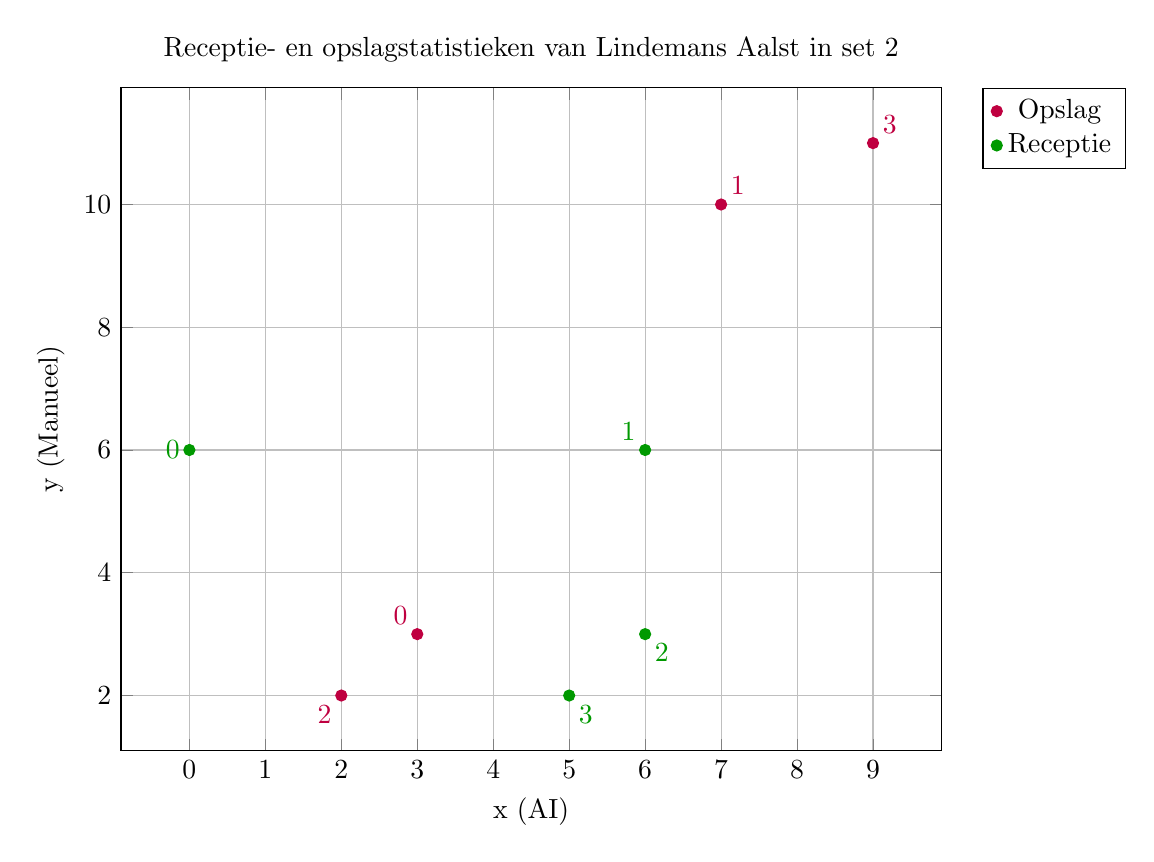
\begin{tikzpicture}
  \begin{axis}[
    title={Receptie- en opslagstatistieken van Lindemans Aalst in set 2},
    xlabel={x (AI)},
    ylabel={y (Manueel)},
    grid=major,
    legend style={at={(1.05,1)}, anchor=north west},
    width=12cm,
    height=10cm,
    enlargelimits=0.1,
  ]

  % Opslag
  \addplot[
    only marks,
    mark=*,
    color=purple,
  ] table {
    x y
    3 3
    7 10
    2 2
    9 11
  };
  \addlegendentry{Opslag}

  % Labels opslag
  \node at (axis cs:3,3) [anchor=south east, purple] {0};
  \node at (axis cs:7,10) [anchor=south west, purple] {1};
  \node at (axis cs:2,2) [anchor=north east, purple] {2};
  \node at (axis cs:9,11) [anchor=south west, purple] {3};

  % Receptie
  \addplot[
    only marks,
    mark=*,
    color=green!60!black,
  ] table {
    x y
    5 2
    6 3
    6 6
    0 6
  };
  \addlegendentry{Receptie}

  % Labels receptie
  \node at (axis cs:5,2) [anchor=north west, green!60!black] {3};
  \node at (axis cs:6,3) [anchor=north west, green!60!black] {2};
  \node at (axis cs:6,6) [anchor=south east, green!60!black] {1};
  \node at (axis cs:0,6) [anchor=east, green!60!black] {0};

  \end{axis}
\end{tikzpicture}
\caption{AI invoer versus manuele invoer, ingedeeld in opslag en receptie, voor Lindemans Aalst in set 2.}
\label{fig:PL1ServeReceiveAalst2}
\end{figure}

Tabel \ref{tab:PL1SetAalstMan2}, \ref{tab:PL1DigAalstMan2} en \ref{tab:PL1SetDigAalstAI2} geven de setting en verdediging statistieken van Lindemans Aalst in set 2 weer. De eerste tabel toont de manueel ingevoerde statistieken van de spelverdeling, terwijl de derde tabel de statistieken toont die door Balltime AI zijn gegenereerd. De setting statistieken zijn onderverdeeld in verschillende categorieën, zoals het aantal sets, het percentage fouten en de effectiviteit van de set. Setter Lucas Lorente López heeft in deze set 19 sets gegeven volgens de scouter en 18 volgens de AI. Bij de andere spelers is dit aantal hetzelfde tussen AI en de manuele invoer. Ook hier is er een verschil op de weergave van de statistieken. = komt overeen met een Set Error (SE). Dit is bij beide hetzelfde. De kwaliteit van de set wordt bij de AI niet beoordeeld, waardoor geen verdere vergelijking mogelijk is.

Bij de verdediging is er een groot verschil tussen de AI en de scouter. De AI heeft verschillende verdedigingen niet herkend, terwijl de scouter dit wel heeft gedaan. Dit is te zien bij bijvoorbeeld Hiago Crins, die 3 verdedigingen heeft gegeven, maar de AI heeft er maar 1 herkend.

\begin{table}[ht!]
  \centering
  \scriptsize
    \begin{tabular}{|l|c|c|c|c|c|c|c|c|c|} \hline
      \textbf{Speler} & *E\% & Tot & = & / & - & ! & + & \# \\ \hline
      Timo Lohmus & 0\% & 2 & 1 &  &  &  & 1 &   \\
      Max Schulz & 50\% & 2 &  &  & 1 & & 1 &  \\
      Alvaro Gimeno Rubio & 50\% & 2 &  &  & 1 &  & 1 &   \\ 
      Lucas Lorente López & 100\% & 19 &  &  &  &  & 19 &  \\ \hline
  \end{tabular}
  \caption[Manueel ingevoerde spelverdelingsstatistieken voor Lindemans Aalst in set 2]{\label{tab:PL1SetAalstMan2}Manueel ingevoerde spelverdelingsstatistieken voor Lindemans Aalst in set 2.}
\end{table}

\begin{table}[ht!]
  \centering
  \scriptsize
    \begin{tabular}{|l|c|c|c|c|c|c|c|c|c|}
      \hline
      \textbf{Speler} & *E\% & Tot & = & / & - & ! & + & \# \\ \hline
      Hiago Crins & 0\% & 3 & 1 &  &  & 1 & 1 &  \\ 
      Bert Dufraing & 100\% & 2 &  &  &  &  & 2 &  \\
      Timo Lohmus & 100\% & 1 &  &  &  &  & 1 &  \\
      Max Schulz & 67\% & 3 & 1 & 2 &  &  &  &  \\
      Mihkel Varblane & 67\% & 3 & 1 &  &  &  & 2 &  \\
      Alvaro Gimeno Rubio & 100\% & 2 &  & 1 &  & 1 &  &  \\
      Lucas Lorente López & 0\% & 1 &  &  & 1 &  &  &  \\ \hline
  \end{tabular}
  \caption[Manueel ingevoerde verdedigingsstatistieken voor Lindemans Aalst in set 2]{\label{tab:PL1DigAalstMan2}Manueel ingevoerde verdedigingsstatistieken voor Lindemans Aalst in set 2.}
\end{table}

\begin{table}[ht!]
  \centering
  \scriptsize
  \begin{tabular}{|l|c|c|c|c|c|c|c|} \hline
    \textbf{Speler} & Ast & TA & SE & PCT & DS & DE \\ \hline
    Hiago Crins &  &  &  &  & 1 &  \\
    Bert Dufraing &  &  &  &  & 1 &  \\ 
    Timo Lohmus & 1 & 2 & 1 & 50\% & 1 &  \\
    Max Schulz & 1 & 2 &  & 50\% & 1 & 1 \\
    Mihkel Varblane &  &  &  &  & 2 &  \\
    Alvaro Gimeno Rubio & 0 & 2 &  & 0\% & 3 &  \\
    Lucas Lorente López & 10 & 18 &  & 56\% & 1 &  \\ \hline
  \end{tabular}
  \caption[Spelverdelings- en verdedigingsstatistieken gemaakt door Balltime AI voor Lindemans Aalst in set 2]{\label{tab:PL1SetDigAalstAI2}Spelverdelings- en verdedigingsstatistieken gemaakt door Balltime AI voor Lindemans Aalst in set 2.}
\end{table}

Bij de aanval (tabel \ref{tab:PL1AttAalstMan2} en \ref{tab:PL1AttBlockAalstAI2}) is het totaal aantal aanvallen gelijk bij iedereen behalve één speler. Hij heeft een aanval minder gekregen door de AI. 

Bij de blokstatistieken (tabel \ref{tab:PL1BlockAalstMan2} en \ref{tab:PL1AttBlockAalstAI2}) wordt er op een volledig andere manier naar gekeken. De AI geeft statistieken waar de speler deel kan zijn van een éénmans- of een meermansblok. Dit is bij de manuele invoer niet het geval. Hierdoor geeft de AI dus eigenlijk ook geen blokpunten aan de spelers. Ookal is dit wel belangrijke informatie.

De aanvallen en bloks worden door de AI niet beoordeeld op kwaliteit.

\begin{table}[ht!]
  \centering
  \scriptsize
    \begin{tabular}{|l|c|c|c|c|c|c|c|c|c|}
      \hline
      \textbf{Speler} & *E\% & Tot & = & / & - & ! & + & \# \\ \hline
      Hiago Crins  & 0\% & 1 &  &  &  &  & 1 &  \\ 
      Timo Lohmus  & 17\% & 6 & 1 &  & 1 & 1 & 1 & 2 \\ 
      Max Schulz  & 22\% & 9 & 1 & 2 &  & 1 & 0 & 5\\
      Mihkel Varblane  & 100\% & 2 &  &  &  &  &  & 2 \\ 
      Alvaro Gimeno Rubio & 29\% & 7 & 1 & 1 &  &  & 1 & 4 \\ \hline 
  \end{tabular}
\caption[Manueel ingevoerde aanvalsstatistieken voor Lindemans Aalst in set 2]{\label{tab:PL1AttAalstMan2}Manueel ingevoerde aanvalsstatistieken voor Lindemans Aalst in set 2.}
\end{table}

\begin{table}[ht!]
  \centering
  \scriptsize
    \begin{tabular}{|l|c|c|c|c|c|c|c|c|c|}
      \hline
      \textbf{Speler} & *E\% & Tot & = & / & - & ! & + & \# \\ \hline
      Hiago Crins & -25\% & 4 & 1 &  & 2 & 1 &  &  \\ 
      Max Schulz & 0\% & 1 &  &  &  & 1 &  & \\
      Mihkel Varblane & 33\% & 3 &  &  & 1 &  & 1 & 2 \\
      Alvaro Gimeno Rubio & -50\% & 2 &  & &  &  & 1 &  \\
      Lucas Lorente López & 0\% & 1 &  &  & 1 &  &  &  \\ \hline
  \end{tabular}
\caption[Manueel ingevoerde blokstatistieken voor Lindemans Aalst in set 2]{\label{tab:PL1BlockAalstMan2}Manueel ingevoerde blokstatistieken voor Lindemans Aalst in set 2.}
\end{table}

\begin{table}[ht!]
  \centering
  \scriptsize
  \begin{tabular}{|l|c|c|c|c|c|c|c|c|c|c|c|} \hline
    \textbf{Speler} & K & E & TA & Atk\% & Kill\%  & Error\% & BS & BA & BE \\ \hline
    Hiago Crins & & & 1 & 0.00 & 0\%  & 0\% & 1 & 1 &\\
    Timo Lohmus & 3 & 1 & 6 & 0.33 & 50\%  & 17\% &  &  & \\
    Max Schulz & 5 & 3 & 9 & 0.22 & 56\%  & 33\% &  & 2 &  \\
    Mihkel Varblane & 2 & 0 & 2 & 1.00 & 100\%  & 0\% & 1 & 1 &  \\
    Alvaro Gimeno Rubio & 3 & 2 & 6 & 0.17 & 50\%  & 33\% &  & 1 & \\
    Lucas Lorente López &  &  &  &  &  &  &  & 1 & \\ \hline
  \end{tabular}
  \caption[Aanvals- en blokstatistieken gemaakt door Balltime AI voor Lindemans Aalst in set 2]{\label{tab:PL1AttBlockAalstAI2}Aanval en blokstatistieken gemaakt door Balltime AI voor Lindemans Aalst in set 2.}
\end{table}
